\begin{figure}[!h]
\begin{minipage}{0.45\textwidth}
    \centering
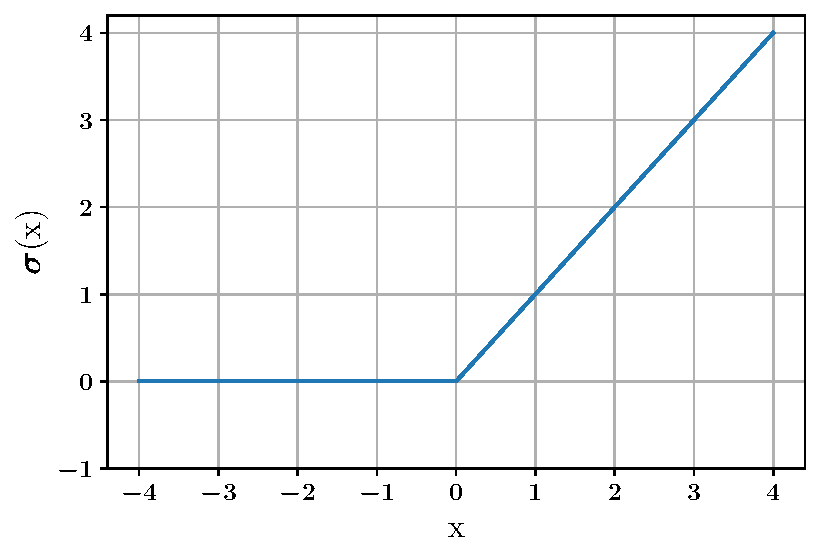
\includegraphics[width=\textwidth]{images/networks/act_relu.pdf}
\caption{ReLU activation function}
    \label{fig:act_relu}
\end{minipage}
\hfill
\begin{minipage}{0.5\textwidth}
    \textbf{Rectified Linear Unit (ReLU)}
   \begin{align}
        a(x) &=
        \begin{cases}
        x   & \text{if } x > 0 \\
        0  & \text{if } x \leq 0 
  \end{cases}
\end{align}
The ReLU is a continuous function with a point of non differentiability in 0. Despite being non differentiable this function is still implemented, mostly in the hidden layers of a network, due to its fast computation time. 
\end{minipage}
\end{figure}

\begin{figure}[!h]
\begin{minipage}{0.45\textwidth}
    \centering
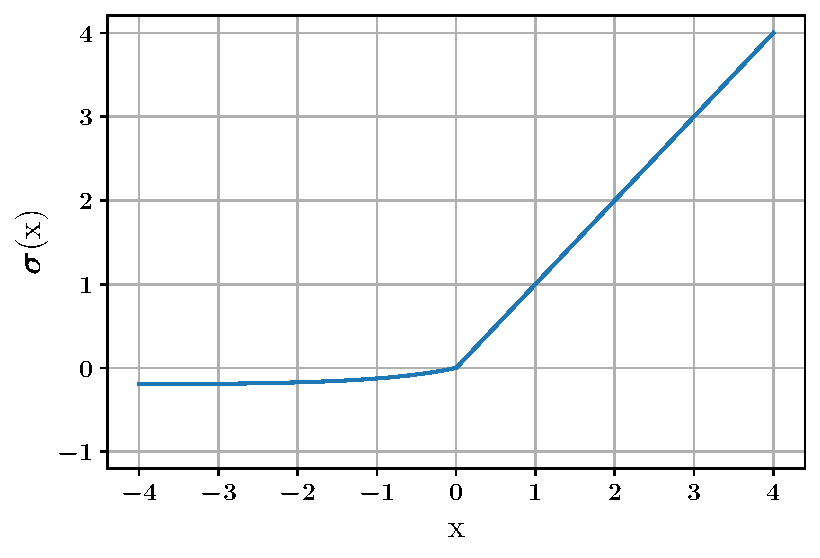
\includegraphics[width=\textwidth]{images/networks/act_elu.pdf}
\caption{ELU activation function}
    \label{fig:elu}
\end{minipage}
\hfill
\begin{minipage}{0.5\textwidth}
    \textbf{Exponential Linear Unit (ELU)}
   \begin{align}
        a(x) &= 
        \begin{cases}
        \alpha \left(e^x -1\right)  & \text{if } x \leq 0 \\
        x  & \text{if } x > 0 
  \end{cases}
\end{align}
The ELU activation functions is an improvement over the ReLU. In this case the negative values have an actual activation instead of being set to zero which may help the estimation of the network parameters. The drawback of choosing this function in an increase in the computational cost since an exponential operation is included. 
\end{minipage}
\end{figure}

\begin{figure}[!h]
\begin{minipage}{0.45\textwidth}
    \centering
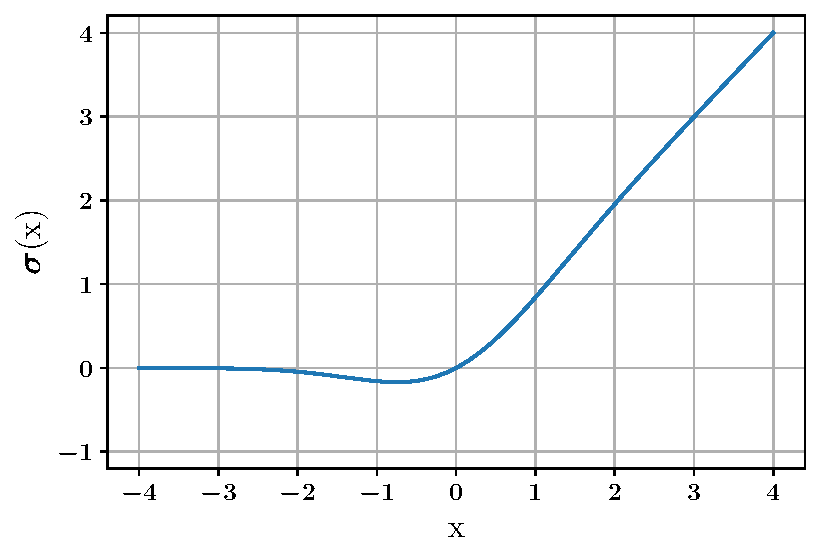
\includegraphics[width=\textwidth]{images/networks/act_gelu.pdf}
\caption{GELU activation function}
    \label{fig:gelu}
\end{minipage}
\hfill
\begin{minipage}{0.5\textwidth}
    \textbf{Gaussian Error Linear Unit (GELU)}
   \begin{equation}
       a(x) = \frac{1}{2} x \left( 1+\text{erf} \left( \frac{x}{\sqrt{2}}\right)\right)
   \end{equation}
   This is one of the newest activation functions. It was implemented in some of the most recent Deep Learining application proving to be one of the best activations in the Natural Language Processing field. 
\end{minipage}
\end{figure}

\begin{figure}[!h]
\begin{minipage}{0.45\textwidth}

    \centering
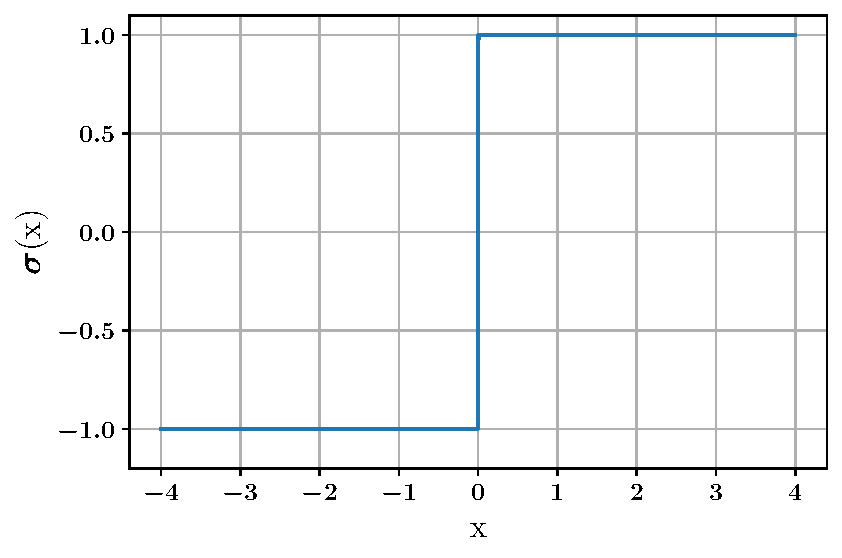
\includegraphics[width=\textwidth]{images/networks/act_step.pdf}
\caption{Step activation function}
    \label{fig:act_step}
\end{minipage}
\hfill
\begin{minipage}{0.5\textwidth}
    \textbf{Binary step}
      \begin{align}
        a(x) &=
        \begin{cases}
        1   & \text{if } x \geq 0 \\
        -1  & \text{if } x < 0 
  \end{cases}
\end{align}
Neurons using this function are also called linear threshold units(LTU). This type of neurons can be used for solving simple tasks but is not able to solve complex tasks like multiclass classifications or image recognitions.
\end{minipage}
    \end{figure}

\begin{figure}[!h]
\begin{minipage}{0.45\textwidth}

    \centering
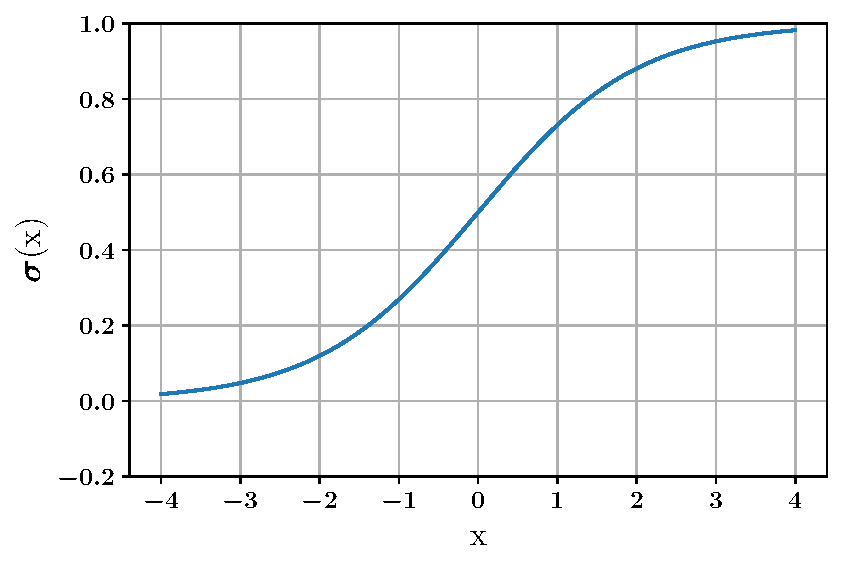
\includegraphics[width=\textwidth]{images/networks/act_sig.pdf}
\caption{Sigmoid activation function}
    \label{fig:act_sig}
\end{minipage}
\hfill
\begin{minipage}{0.5\textwidth}
    \textbf{Sigmoid} or \textbf{Soft step}
   \begin{equation}
       a(x) =\frac{1}{1+e^{-x}}
   \end{equation}
   The sigmoid functions provides an output value in $[0,1]$ and is differentiable in every point. This properties makes it one of the most used activation functions for the last layer of an ANN.
\end{minipage}
    \end{figure}


\begin{figure}[!h]
\begin{minipage}{0.45\textwidth}
    \centering
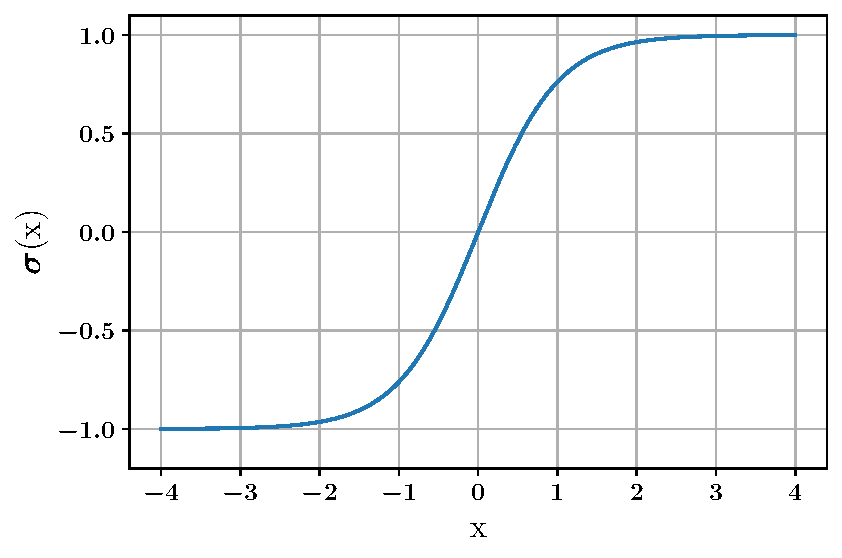
\includegraphics[width=\textwidth]{images/networks/act_tanh.pdf}
\caption{Hyperbolic tangent activation function}
    \label{fig:act_tanh}
\end{minipage}
\hfill
\begin{minipage}{0.5\textwidth}
    \textbf{Hyperbolic tangent}
   \begin{equation}
       a(x) =\frac{e^x-e^{-x}}{e^x+e^{-x}}
   \end{equation}
The hyperbolic tangent has similar properties to the sigmoid function. Its output is however in $[-1,1]$ which may speed up convergence in same applications.
\end{minipage}
\end{figure}